\section{Aktualisierung von Transformationsfolgen}
\label{sec:merging}
Dieser Abschnitt behandelt das Aktualisieren von Transformationsfolgen, welches aufgrund der jährlichen Änderungen im MeSH notwendig ist, wie in \ref{sec:anual_changes} \nameref{sec:anual_changes} beschrieben.

\subsection{Problembeschreibung}
Das Aktualisierungsproblem ist in \autoref{fig:anualChangesStructure} dargestellt. Es folgt eine formalere Beschreibung:

\begin{itemize}
\item[]Seien \code{S} und \code{T} zwei MeSH-Graphen.\par

Sei \code{O} eine Folge von Transformationen, so dass \code{O(S)} = \code{S'}.\par

Gesucht ist eine Folge von Transformationen \code{O'}, so dass \code{O'(T)} = \code{T'}. Dabei soll das semantische Ergebnis der Anwendung von \code{O} auf \code{S} und \code{O'} auf \code{T} möglichst ähnlich sein.\par  
\end{itemize}

%"`ähnlich"' ist hier ein schwammiger Begriff, der sich nicht in Definitionen packen lässt.
Der Semedico-MeSH wurde nach den Erfordernissen von Semedico erstellt, wurde in diesem Sinne also nach semantischen Kriterien aus der Gesamtheit des MeSH ausgewählt. Man hat bestimmte Teile des MeSH so ausgewählt und neu angeordnet, wie es für Semedico aus inhaltlichen Gründen sinnvoll ist. Das Ziel ist es nun diese Semantik der Auswahl über die jährlichen Veränderungen des MeSHs hinaus zu erhalten -- allerdings ausschließlich auf Basis von strukturellen Veränderungen. Es findet keine inhaltliche Analyse der Descriptors oder Tree Vertices, auf die die verschiedenen Transformationen angewandt werden, statt. \par

Der Begriff der Ähnlichkeit, wie er oben in der Definition verwendet wurde, wird nachfolgend nur indirekt genauer charakterisiert, nämlich durch das in den folgenden Abschnitten beschriebene Vorgehen zur Aktualisierung der Transformationen. Dieses Vorgehen ist gerade so gewählt, dass eine aktualisierte Transformation möglichst ähnlich zur Ausgangsoperation ist.\par

Dieses Kapitel der Studienarbeit ist damit weniger als wissenschaftliche Arbeit zu sehen. Es ist allein praktisch motiviert, da ein Tool mit eben dieser Funktionalität gebraucht wird, selbst wenn es nur oberflächlich bewertet werden kann: zum einen anhand der Sinnhaftigkeit des Vorgehens und zum anderen anhand einer manuellen, qualitativen Überprüfung des Ergebnisses des Tools.

%Eine andere Formulierung des Problem wäre die folgende: Es gilt eine solche Vereinigung der Transformationsmengen \code{O} und \code{$\Delta$} zu finden, so dass \code{$\Delta$} gar nicht und \code{O} möglichst wenig verändert werden muss.

%.. Wie zuvor werden hier Heuristiken angewandt, die im allgemeinen sinnvoll erscheinen, im Einzelfall aber suboptimal sein können.

\begin{figure}[h]
\begin{center}
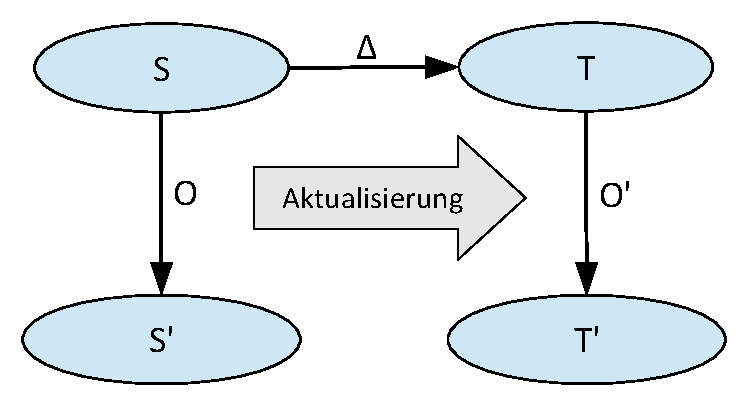
\includegraphics[width=0.6\textwidth]{figs/anualChangesStructure.pdf}
\end{center}
\caption{Aktualisierung der Transformationsfolge \code{O} für einen Ziel-MeSH-Graphen \code{T}}
\label{fig:anualChangesStructure}
\end{figure}

\subsection{Grundidee}
Das Aktualisieren der Transformationen läuft in folgenden Schritten ab:\par

\begin{enumerate}
  \item Bestimmen einer Transformationsfolge \code{$\Delta$}, welche \code{S} in \code{T} überführt
  \item Aktualisieren der Transformationen in \code{O}, als \code{O'}:
  \begin{enumerate}
    \item Descriptor-Additionen
    \item Descriptor-Umbenennungen
    \item Descriptor-Relabellings
    \item Vertex-Additionen
    \item Vertex-Verschiebungen
    \item Vertex-Löschungen
    \item Descriptor-Löschungen
    \item Vertex-Umbenennungen
  \end{enumerate}
\end{enumerate}

Zuerst bestimmen wir \code{$\Delta$}. Diese Informationen über die Änderungen, welche \code{S} in dessen neue Version \code{T} überführen, sind die Grundlage um alle Transformationen aus \code{O} zu aktualisieren. \par

Danach überführen wir alle Transformationen aus \code{O} in ihre für \code{T} angepasste Form in \code{O'}. Die prinzipielle Vorgehensweise ist dabei immer gleich: es wird über alle Transformationen eines Typs iteriert und dabei, für jede Transformation, die in den jeweilig folgenden Unterabschnitten beschriebe Heuristik angewandt. Die so aktualisierte Transformation wird dann \code{O'} hinzugefügt. \par

Die oben gegebene Reihenfolge ist bis auf eine Ausnahme beliebig: Descriptor-Additionen müssen vor Vertex-Additionen aktualisiert werden, da die Aktualisierung der Descriptor-Additionen eine Veränderung der Vertex-Additionen bewirken kann. Die restliche Reihenfolge ist beliebig, da unser konkretes Vorgehen für die verschiedenen Transformationstypen keine wechselseitigen Abhängigkeiten enthält.\par

\subsection{Vorgehen für Aktualisierung einer Transformation}
Die Aktualisierung einer Transformation \code{op} läuft immer nach dem selben Prinzip ab: \par

Man überprüft nacheinander für die einzelnen Parameter \code{op}\,s, ob diese auch in \code{T} vorhanden bzw. gültig sind. Möchte man beispielsweise eine Tree Vertex verschieben, so muss die zu verschiebende Tree Vertex in \code{T} überhaupt vorhanden sein. \par

Ist sie das nicht, wird überprüft, ob eine der Transformationen in \code{$\Delta$} dafür verantwortlich ist. Zum Beispiel könnte die Tree Vertex verschoben oder gelöscht worden sein. Wenn keine passende Transformation aus \code{$\Delta$} gefunden werden kann, wird mit einer Fehlermeldung beendet. Dieser Fall sollte nicht auftreten, da alle Veränderungen an \code{S} von \code{$\Delta$} erfasst sein sollten. Folglich ist entweder \code{$\Delta$} inkorrekt bestimmt worden, oder \code{S} oder \code{T} sind nach dem Berechnen von \code{$\Delta$} verändern worden. \par 

Wenn eine passende Transformation gefunden wurde, ist es unter Umständen möglich das Problem zu beheben. Beispielsweise verschiebt man statt der ursprünglichen, nicht mehr vorhandenen Vertex, die verschobene Vertex. Wenn kein Fix möglich ist, wird eine Fehlermeldung ausgegeben und \code{op} nicht zu \code{O'} hinzugefügt. \par

Da es erstens bei mehr als einem Parameter zu Problemen kommen kann, und zweitens auch ein Fix nicht zwangsweise zu einem gültigen Parameter führt, wiederholt man die Aktualisierung solange, bis entweder ein Fehler auftritt, der nicht gefixt werden kann, oder aber die Transformation durch die angewendeten Fixes gültig geworden ist. In letzterem Fall kann die Transformation nach \code{O'} übernommen werden.

\minisec{Bezeichnungen}
Es folgen Erläuterungen zu den Bezeichnungen in diesem Abschnitt. \par

\begin{tabular}{rl}
   \code{dad(v)} & Vater der Tree Vertex \code{v} \\
   \code{name(d)} & Name eines Descriptors \code{d} \\
   \code{ui(d)} & UI eines Descriptors \code{d} \\ \\
   \code{S(ui)} & Descriptor in \code{S} der UI \code{ui} besitzt\\
   \code{S(dname)} & Descriptor in \code{S} der Name \code{dname} besitzt\\
   \code{S(vname)} & Tree Vertex in \code{S} die Name \code{vname} besitzt\\ 
\end{tabular}  

In den Grafiken sollen die verschiedenen Farben zum Verständnis beitragen: \par
\begin{tabular}{rl}
 gelb & Einstiegspunkt. Zeigt die zu aktualisierende Transformation mit Parametern.\\
 blauer Kreis mit \code{x} & Überprüfung eines Parameters \code{x} ob dieser angepasst werden muss.\\ 
 hellblau & "`Normale"' Bedingungen und Anweisungen. \\
 grün & Erfolgreicher Abschluss der Aktualisierung. \\
 rot & Fehler.
\end{tabular}

\subsubsection{Descriptor-Additionen}

\begin{figure}[h]
\begin{center}
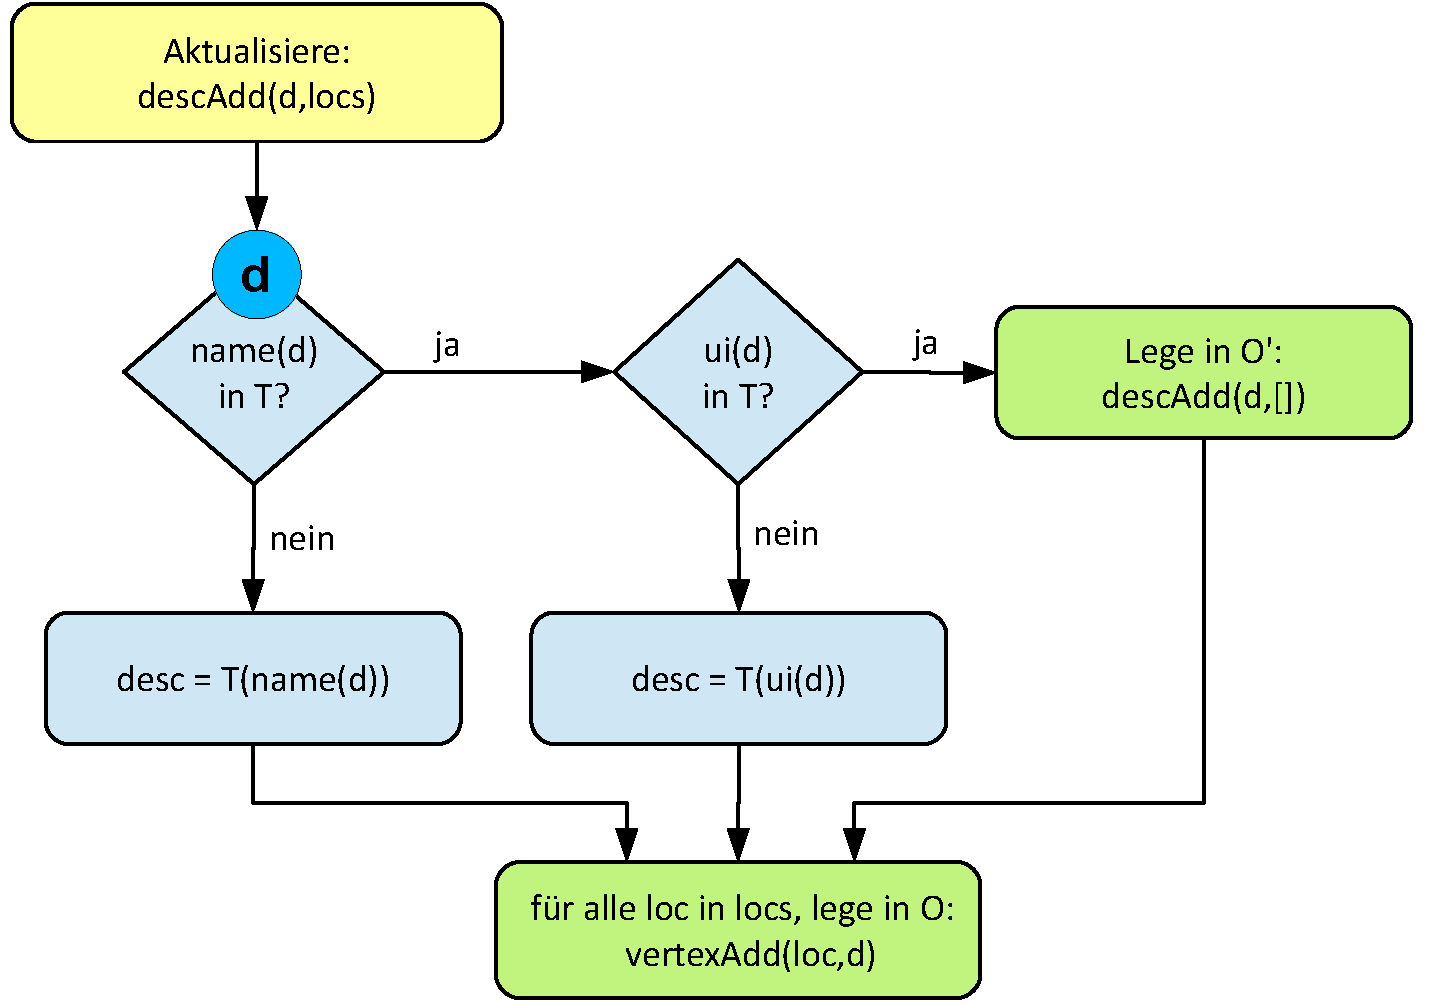
\includegraphics[width=0.8\textwidth]{figs/merge_descAdd.pdf}
\end{center}
\caption{Aktualisierung von Descriptor-Additionen}
\label{figs:merge_descAdd}
\end{figure}

Bei der Aktualisierung des Hinzufügen eines Descriptors werden immer alle Tree Vertices als separate Tree-Vertex-Additionen behandelt und diese zu \code{O} (nicht \code{O'}!) hinzugefügt. Dadurch werden die Tree-Vertex-Additionen später auf mögliche Probleme überprüft.\par

Übrig bleibt das Hinzufügen des Descriptors selbst. Wenn dessen Name oder UI bereits in \code{T} existieren, wird dieser nicht hinzugefügt. Als Descriptor für die hinzuzufügenden Tree Vertices wird dann der Descriptor des bereits existierenden Namens bzw. der bereits existierenden UI verwandt. \par

Wenn weder UI noch Name in \code{T} existieren, kann die Descriptor-Addition nach \code{O'} übernommen werden.

%Das Hinzufügen eines Descriptor muss nur aktualisiert werden, wenn entweder die UI oder der Name des hinzuzufügenden Descriptors in \code{T} bereits existieren. Ist dies der Fall, wird nicht der Descriptor selbst hinzugefügt, sondern nur die Tree Vertices. Der dazugehörige Descriptor ist dann der des bereits existierenden Namens bzw. der bereits existierenden UI. \par  

\subsubsection{Descriptor-Umbenennungen}

\begin{figure}
\begin{center}
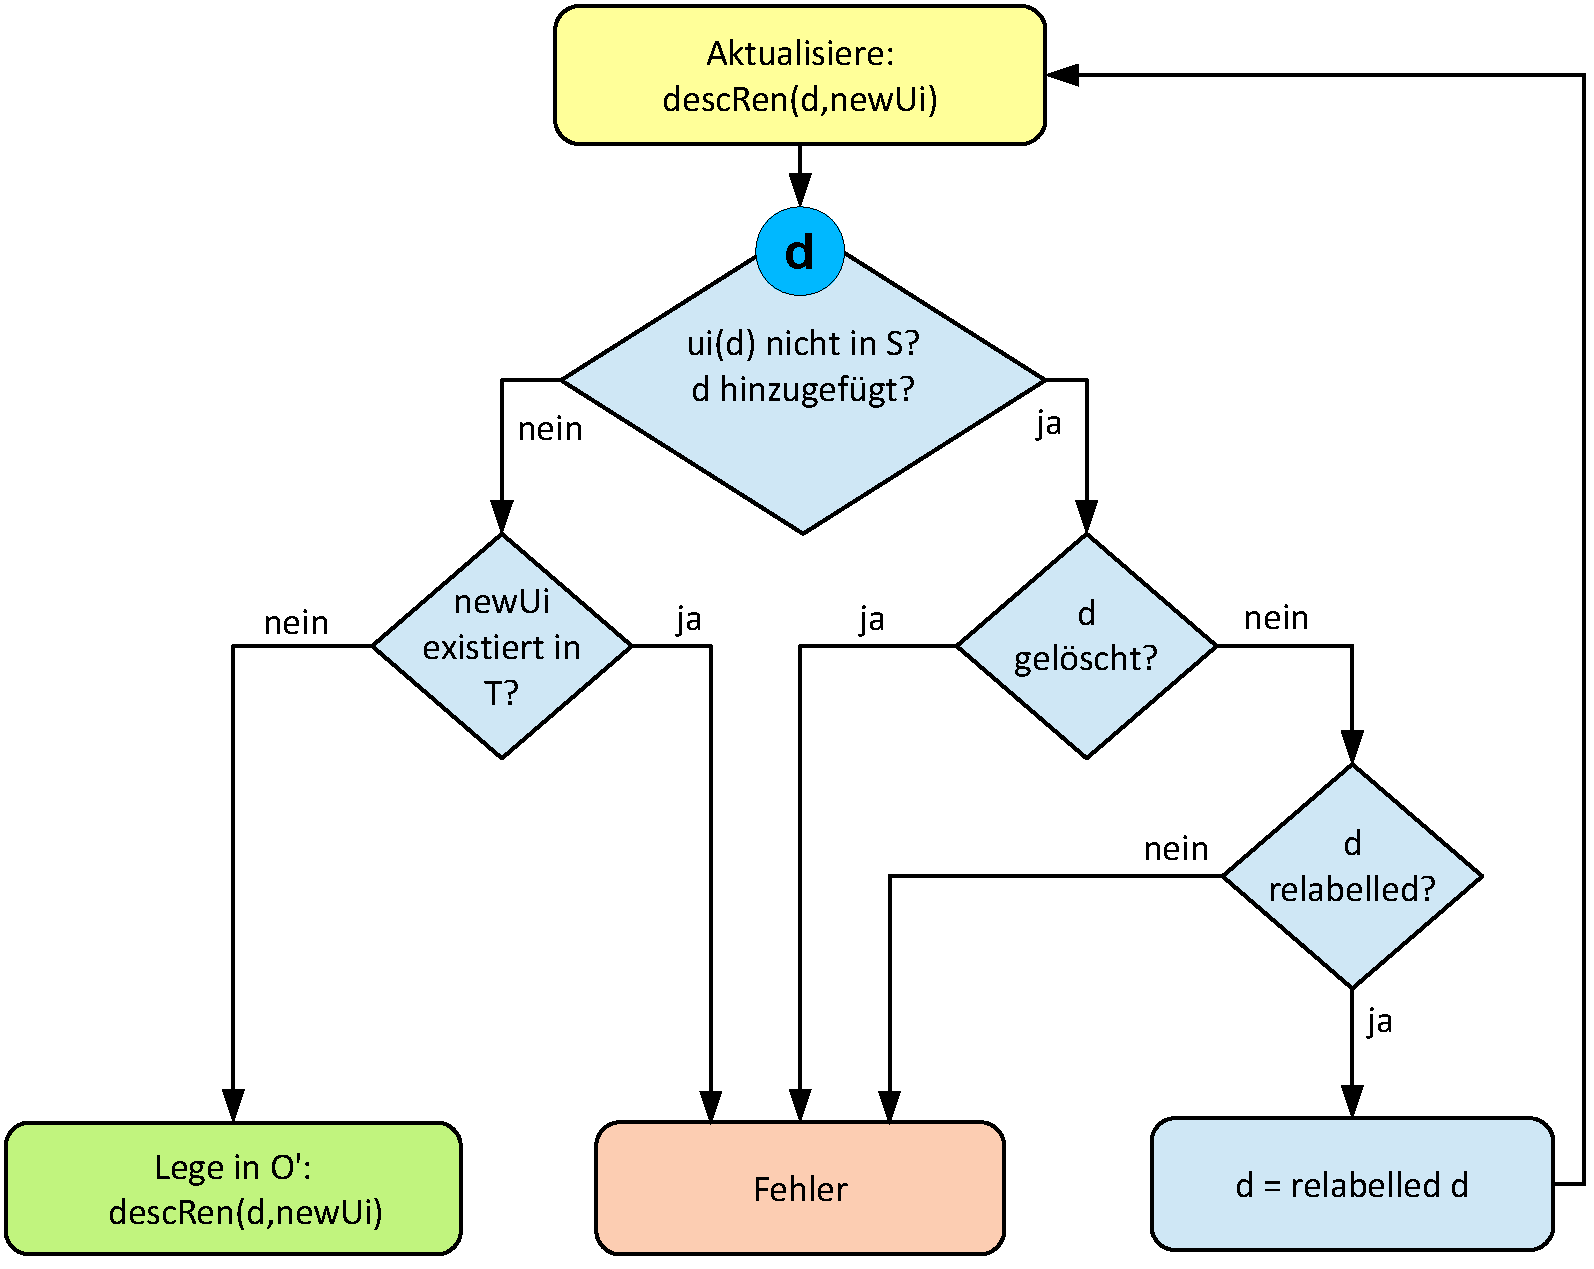
\includegraphics[width=0.9\textwidth]{figs/merge_descRen.pdf}
\end{center}
\caption{Aktualisierung von Descriptor-Umbenennungen}
\label{figs:merge_descRen}
\end{figure}
Siehe \autoref{figs:merge_descRen}.\par

Falls Descriptor \code{desc} in \code{T} bereits existiert, dann kann es zwei logische Ursachen geben:
\begin{enumerate}
  \item Der Descriptor wurde gelöscht. Dann ist eine Aktualisierung der Transformation unmöglich. 
  \item Der Descriptor hat eine andere UI bekommen. Dann verwenden wir diese veränderte UI zur abermaligen Aktualisierung der Transformation.
  \item[] Ansonsten wird ein Fehler gemeldet.
\end{enumerate}

Auch wenn \code{desc} in \code{T} nicht vorhanden ist, kann ein Problem auftreten. Nämlich, wenn die neue UI des Descriptors in \code{T} bereits vorhanden ist. In diesem Fall wird ebenfalls eine Fehlermeldung ausgegeben, da hier nicht klar ist, was getan werden sollte. 

\subsubsection{Vertex-Additionen}
Siehe \autoref{figs:merge_vertexAdd}.\par

Falls der Descriptor, zu dem eine Vertex hinzugefügt werden soll, umbenannt wurde, dann wird versucht die Vertex zu dem umbenannten Descriptor hinzuzufügen. \par

Wurde der Descriptor hingegen gelöscht, ist kein Weiterkommen und ein Fehler wird gemeldet. \par

Kann der \code{p} nicht gefunden werden, weil es gelöscht wurde, so wird stattdessen versucht \code{v} als Kind von \code{dad(p)} einzufügen. \par
 
Wenn \code{p} umbenannt wurde, fügen wir \code{v} als Kind dieser umbenannten Tree Vertex ein.

\begin{figure}
\begin{center}
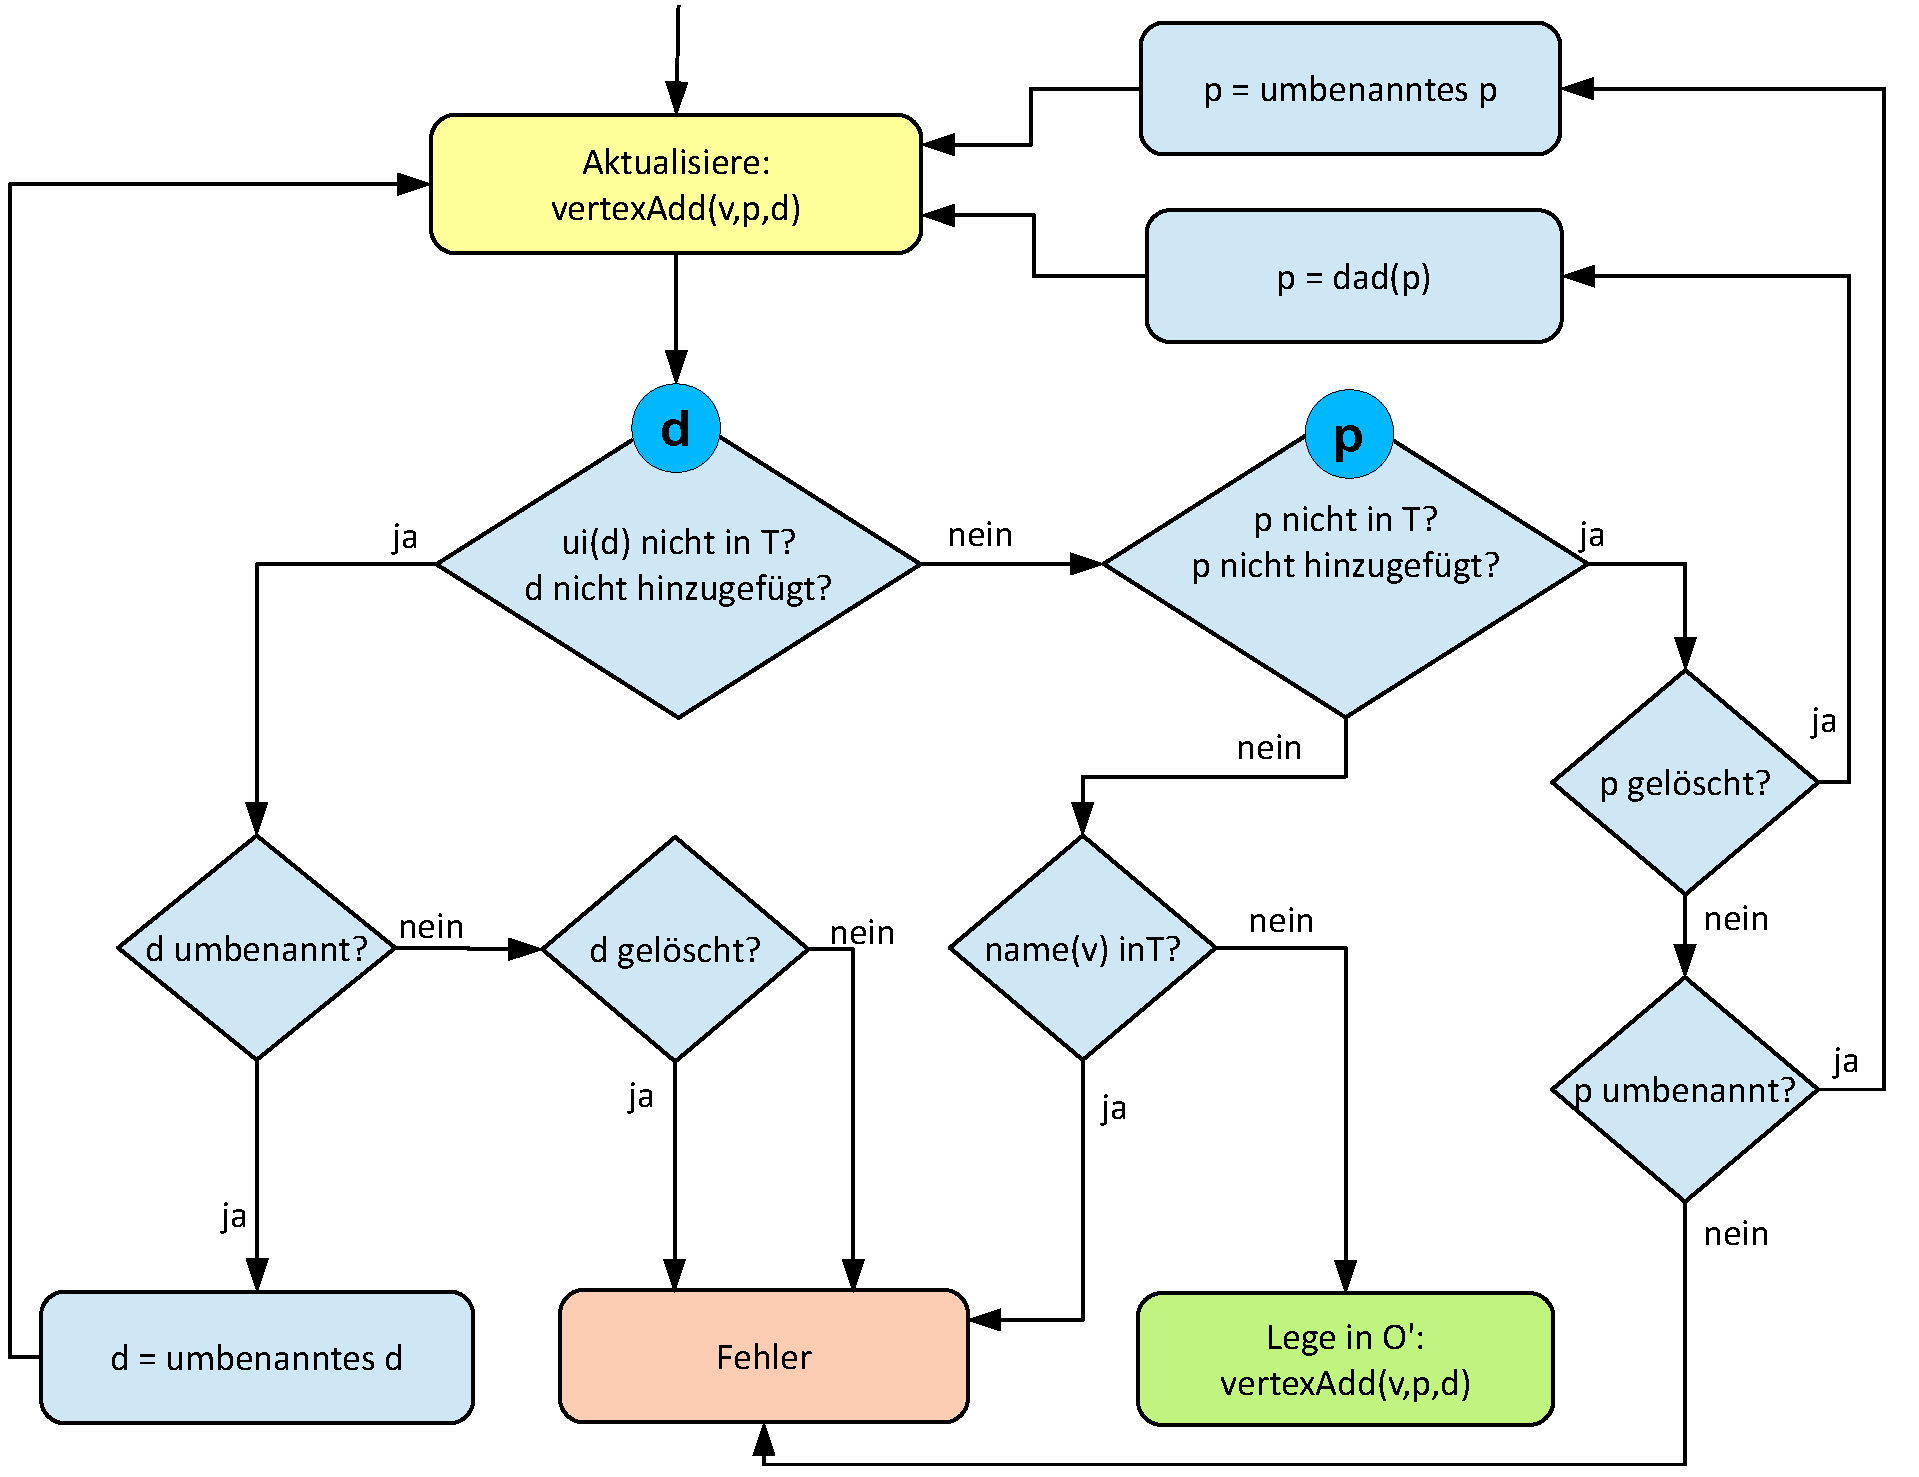
\includegraphics[width=1.1\textwidth]{figs/merge_vertexAdd.pdf}
\end{center}
\caption{Aktualisierung von Vertex-Additionen}
\label{figs:merge_vertexAdd}
\end{figure}

\subsubsection{Vertex-Verschiebungen}
Da \code{vertexMove} viele Parameter besitzt und dadurch die Grafik zu groß werden würde, ist sie in eine Übersichtsgrafik (\autoref{figs:merge_vertexMove_overview}) und 4 Teilgrafiken (\autoref{figs:merge_vertexMove_1} bis \autoref{figs:merge_vertexMove_4}) aufgeteilt worden: eine Grafik für die Problembehandlung eines jeden Parameters. \par

Die Abfragen \code{"`Aktualisierung durch x?"'} in \autoref{figs:merge_vertexMove_overview} entsprechen dem Test, ob ein Parameter \code{x} in \code{T} nicht vorhanden ist und auch nicht durch eine Transformation aus \code{$\Delta$} hinzugefügt wurde.

\begin{figure}
\begin{center}
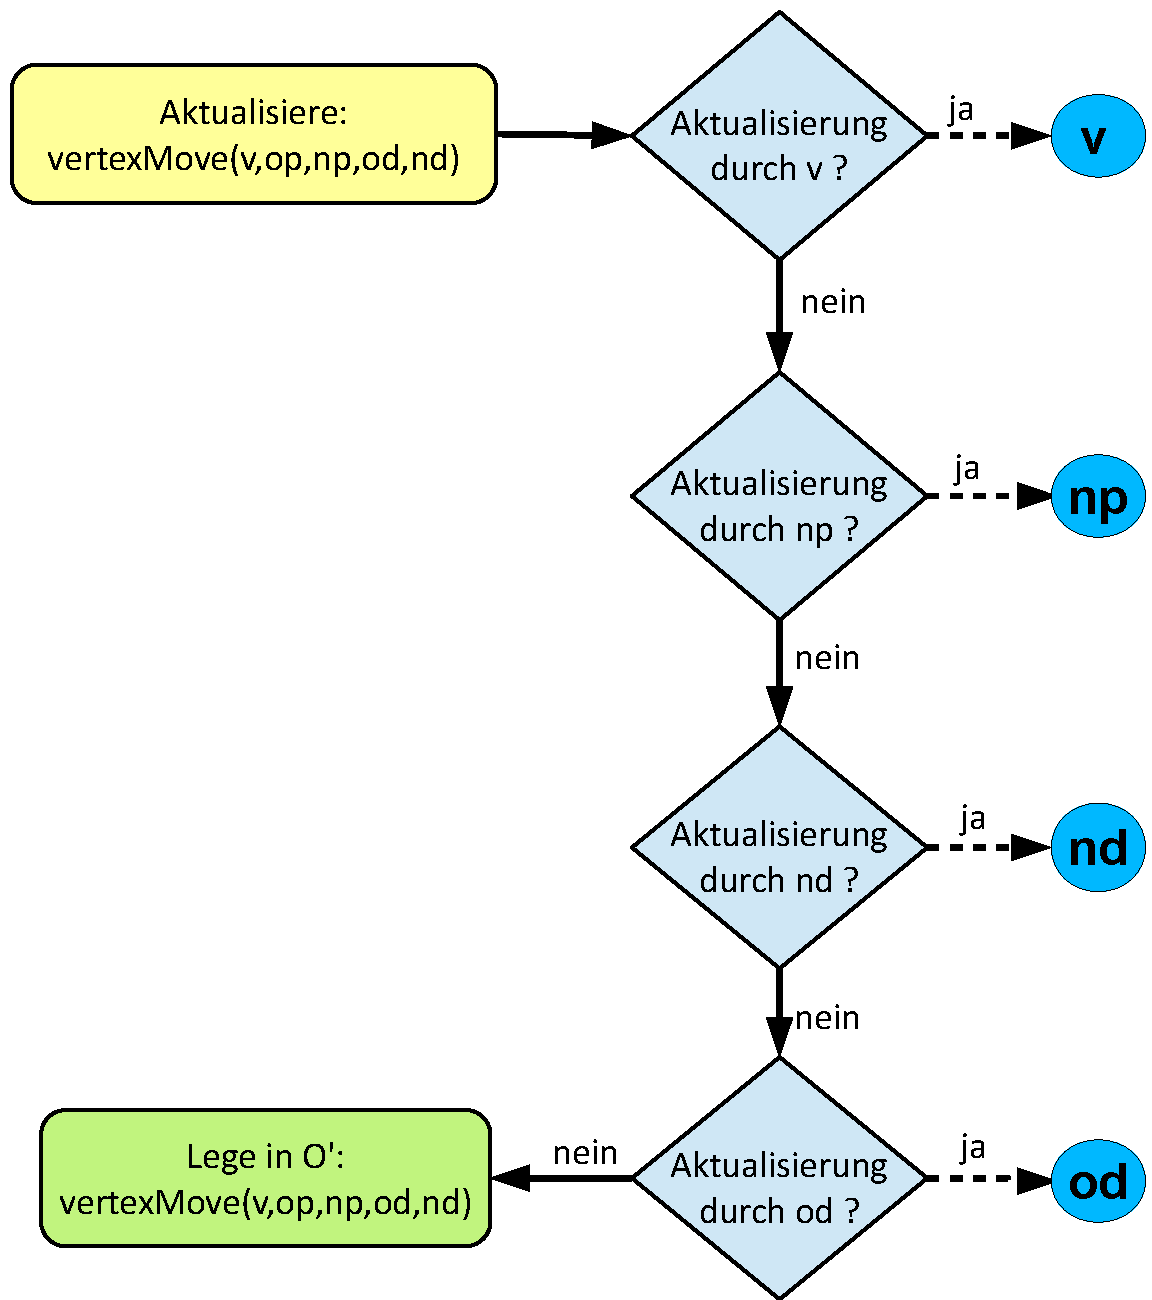
\includegraphics[width=0.6\textwidth]{figs/merge_vertexMove_overview.pdf}
\end{center}
\caption{Aktualisierung von Vertex-Verschiebungen - Übersicht}
\label{figs:merge_vertexMove_overview}
\end{figure}

Die Grafiken \autoref{figs:merge_vertexMove_1}, \autoref{figs:merge_vertexMove_2}, \autoref{figs:merge_vertexMove_3} und \autoref{figs:merge_vertexMove_4} sind weitgehend selbsterklärend. Daher folgen nur Erläuterungen zu den Schlüsselstellen. \par

\begin{figure}
\begin{center}
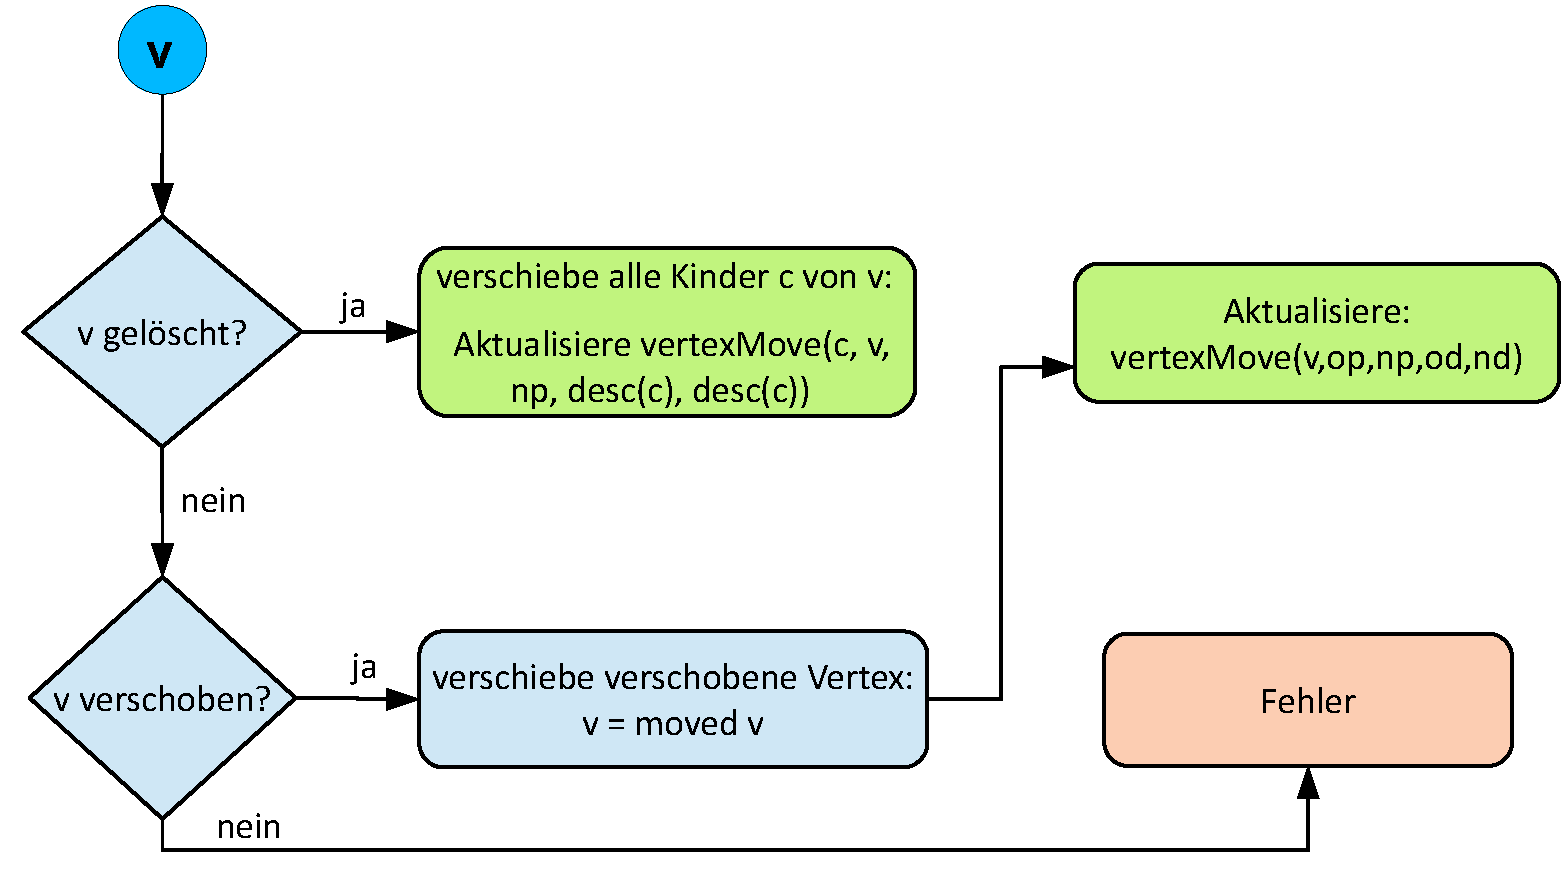
\includegraphics[width=0.7\textwidth]{figs/merge_vertexMove_1.pdf}
\end{center}
\caption{Vertex-Verschiebungen - Veränderungen an \code{v}}
\label{figs:merge_vertexMove_1}
\end{figure}

\begin{figure}
\begin{center}
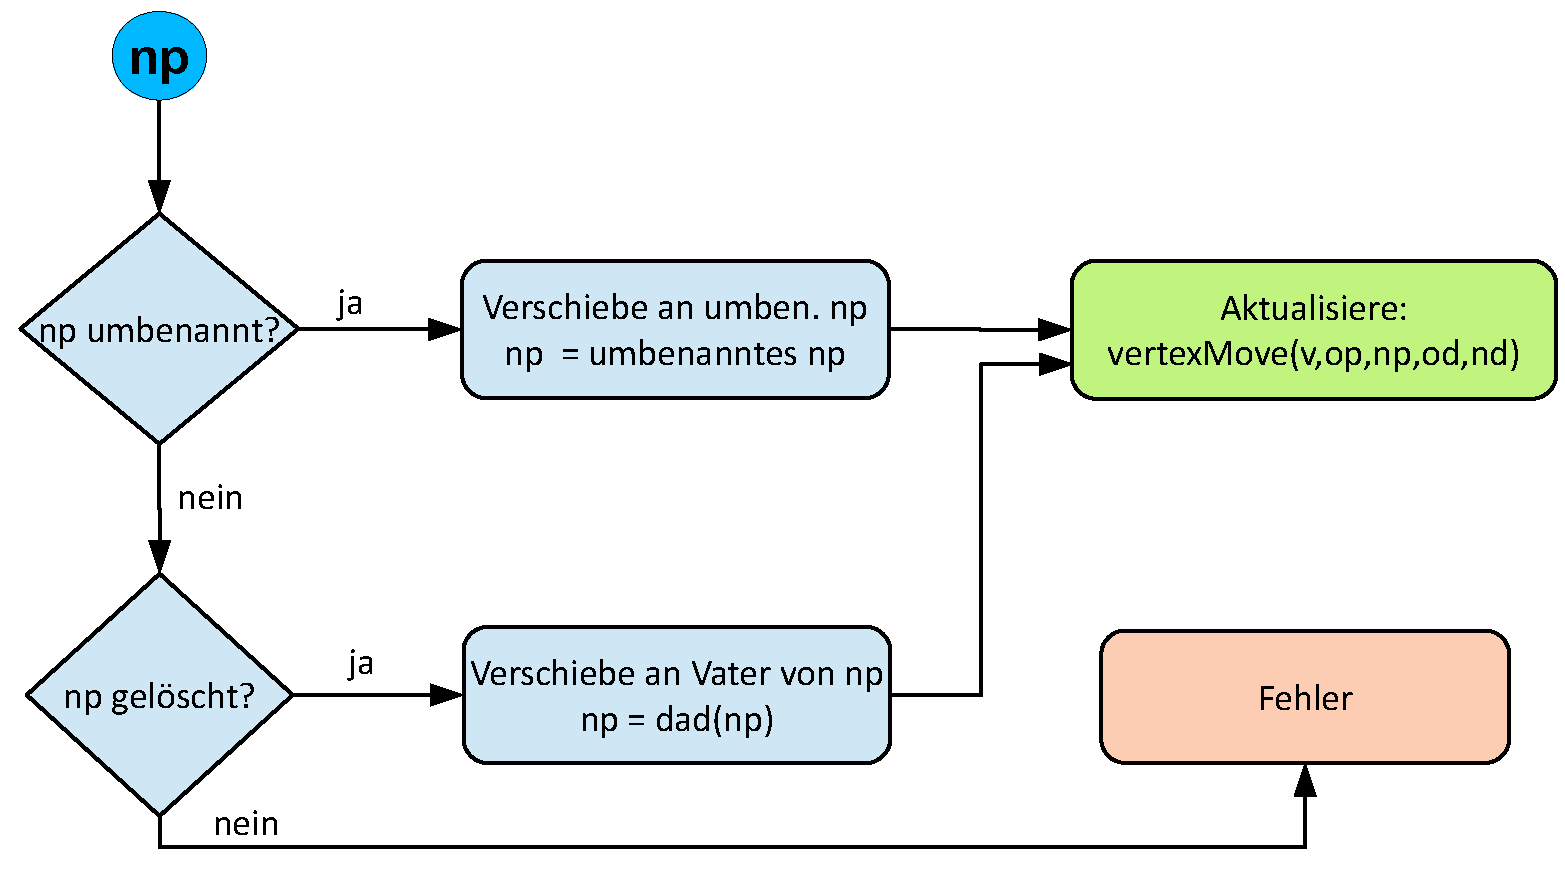
\includegraphics[width=0.7\textwidth]{figs/merge_vertexMove_2.pdf}
\end{center}
\caption{Vertex-Verschiebungen - Veränderungen an \code{np}}
\label{figs:merge_vertexMove_2}
\end{figure}

\begin{figure}
\begin{center}
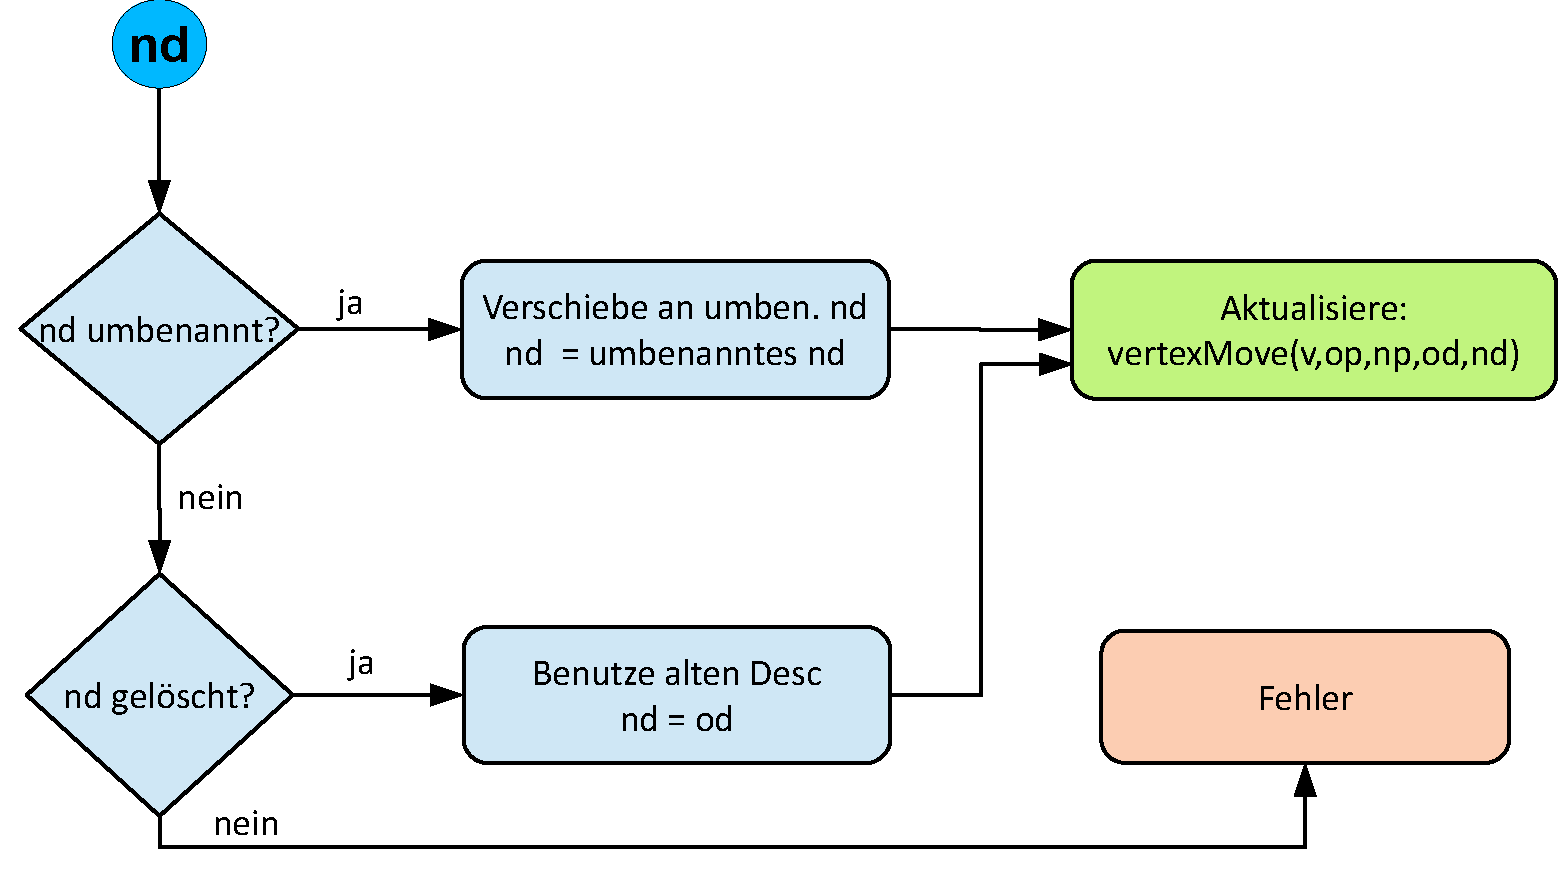
\includegraphics[width=0.7\textwidth]{figs/merge_vertexMove_3.pdf}
\end{center}
\caption{Vertex-Verschiebungen - Veränderungen an \code{nd}}
\label{figs:merge_vertexMove_3}
\end{figure}

\autoref{figs:merge_vertexMove_3}: Falls der neue Descriptor \code{nd} aus \code{T} gelöscht wurde, wird als Fix stattdessen der alte Descriptor \code{od} verwendet. Dies ist sinnvoll, da das explizite Verschieben \code{v}\,s impliziert, dass \code{v} für Semedico wichtig ist. Anstatt hier also mit einer Fehlermeldung abzubrechen, wird versucht die Transformation zu erhalten.

\begin{figure}
\begin{center}
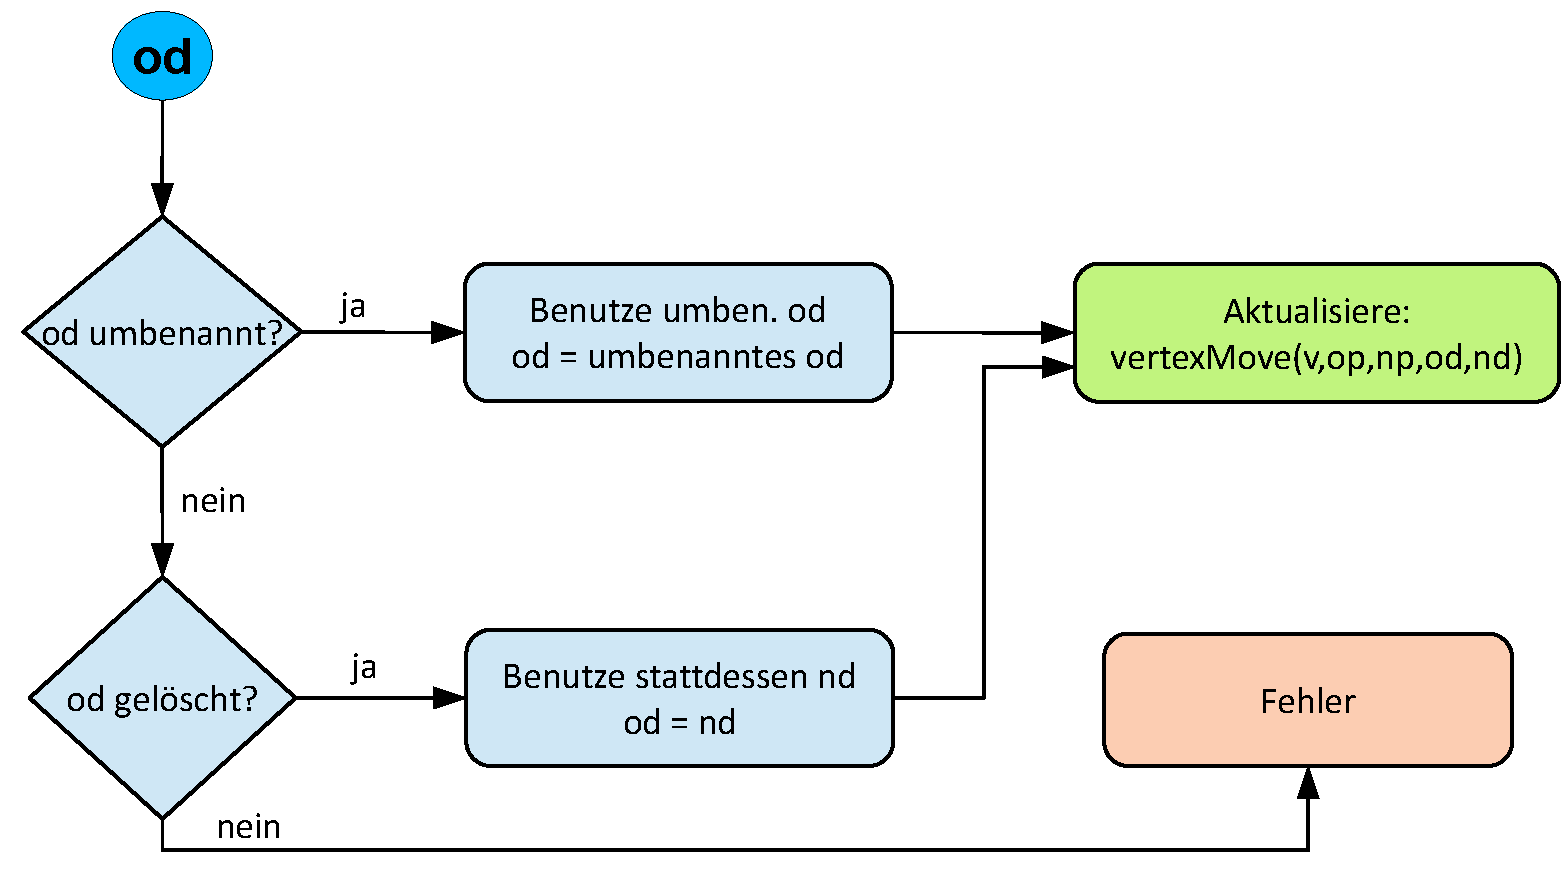
\includegraphics[width=0.7\textwidth]{figs/merge_vertexMove_4.pdf}
\end{center}
\caption{Vertex-Verschiebungen - Veränderungen an \code{od}}
\label{figs:merge_vertexMove_4}
\end{figure}

\autoref{figs:merge_vertexMove_3}: Falls der alte Descriptor \code{od} aus \code{T} gelöscht wurde, wird als Fix stattdessen der neue Descriptor \code{od} verwendet. \code{od} wird nur benötigt, um \code{od}, im Falle einer Vertex-Neuverknüpfung \code{v}\,s, zu informieren, dass \code{od} eine Tree Vertex verloren hat. Da \code{od} aber entfernt wurde, wird diese Information nicht länger benötigt und es ist korrekt \code{od} auf \code{nd} zu setzen.

\subsubsection{Vertex-Löschungen}

Siehe \autoref{figs:merge_vertexDel}. \par

Das Vorgehen ist eingängig: ist \code{v} unverändert vorhanden, kann die Vertex-Löschung direkt übernommen werden. Wurde \code{v} gelöscht, muss entweder nichts mehr getan werden, falls die Löschung nicht rekursiv war, oder es wird als Fix versucht alle Kinder \code{v}\,s zu löschen. Wurde \code{v} hingegen verschoben, so wird versucht verschobene Tree Vertex zu löschen. 

\begin{figure}
\begin{center}
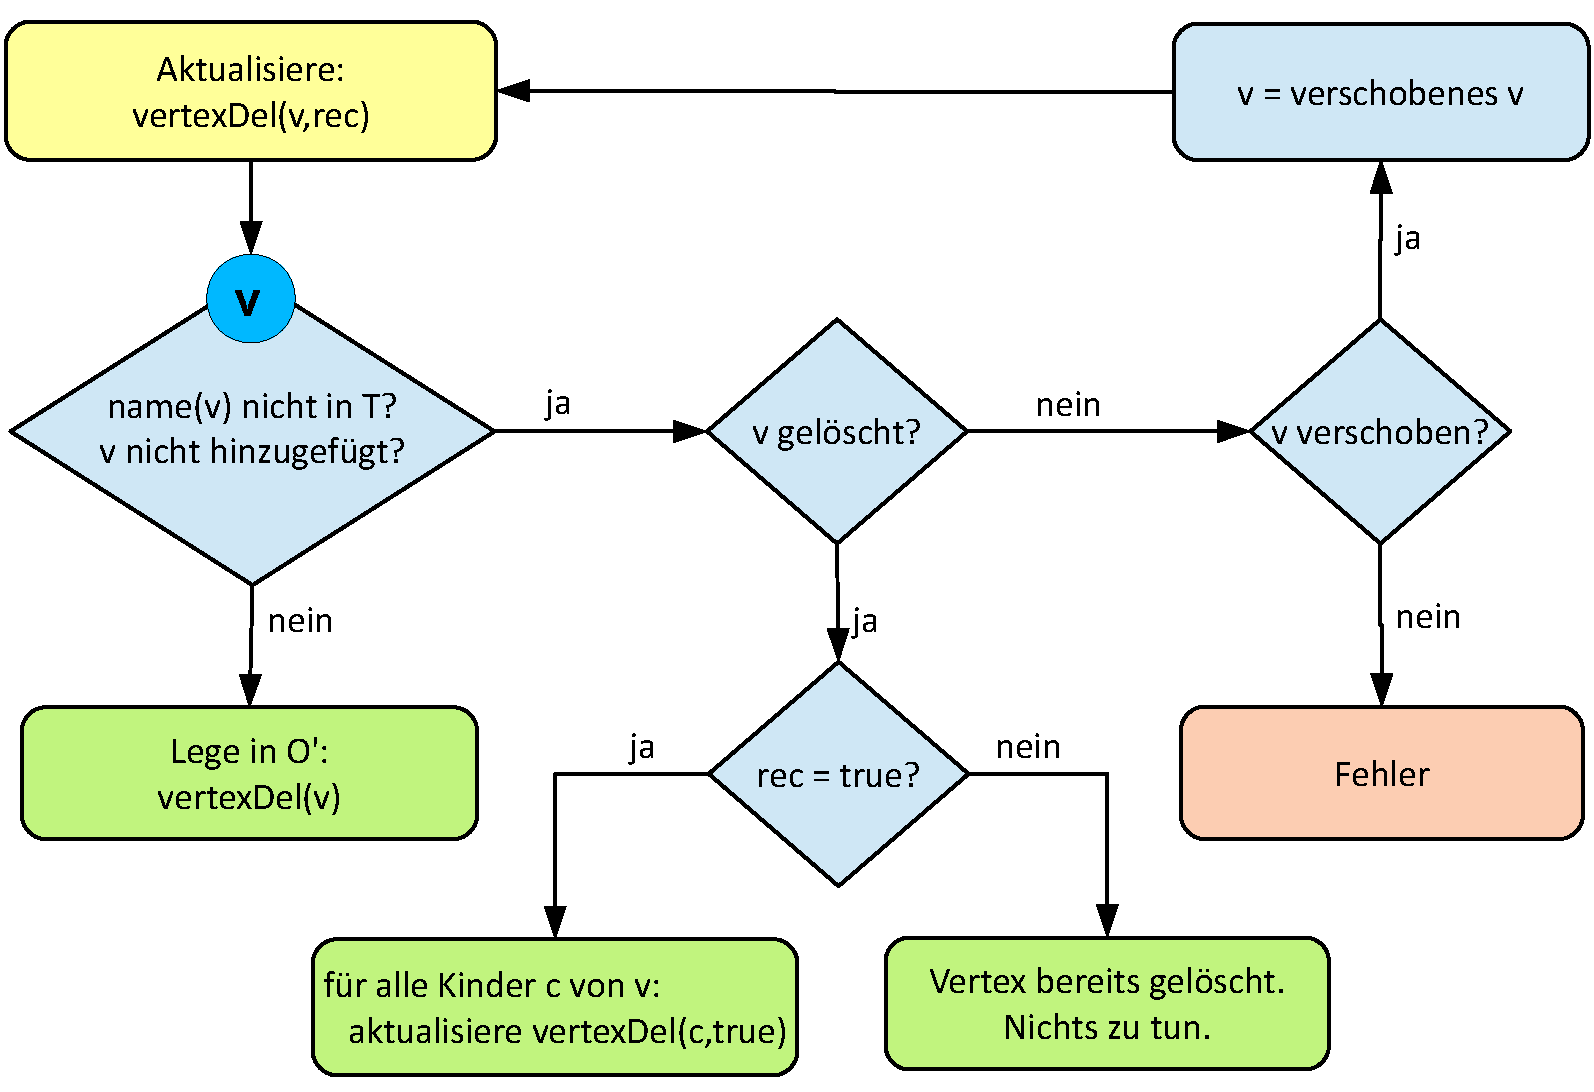
\includegraphics[width=0.80\textwidth]{figs/merge_vertexDel.pdf}
\end{center}
\caption{Aktualisierung von Vertex-Löschungen}
\label{figs:merge_vertexDel}
\end{figure}

\subsubsection{Descriptor-Löschungen}

Siehe \autoref{figs:merge_descDel}. \par 
Das Vorgehen hier ist weitgehend analog zu dem für Vertex-Löschungen.

\begin{figure}
\begin{center}
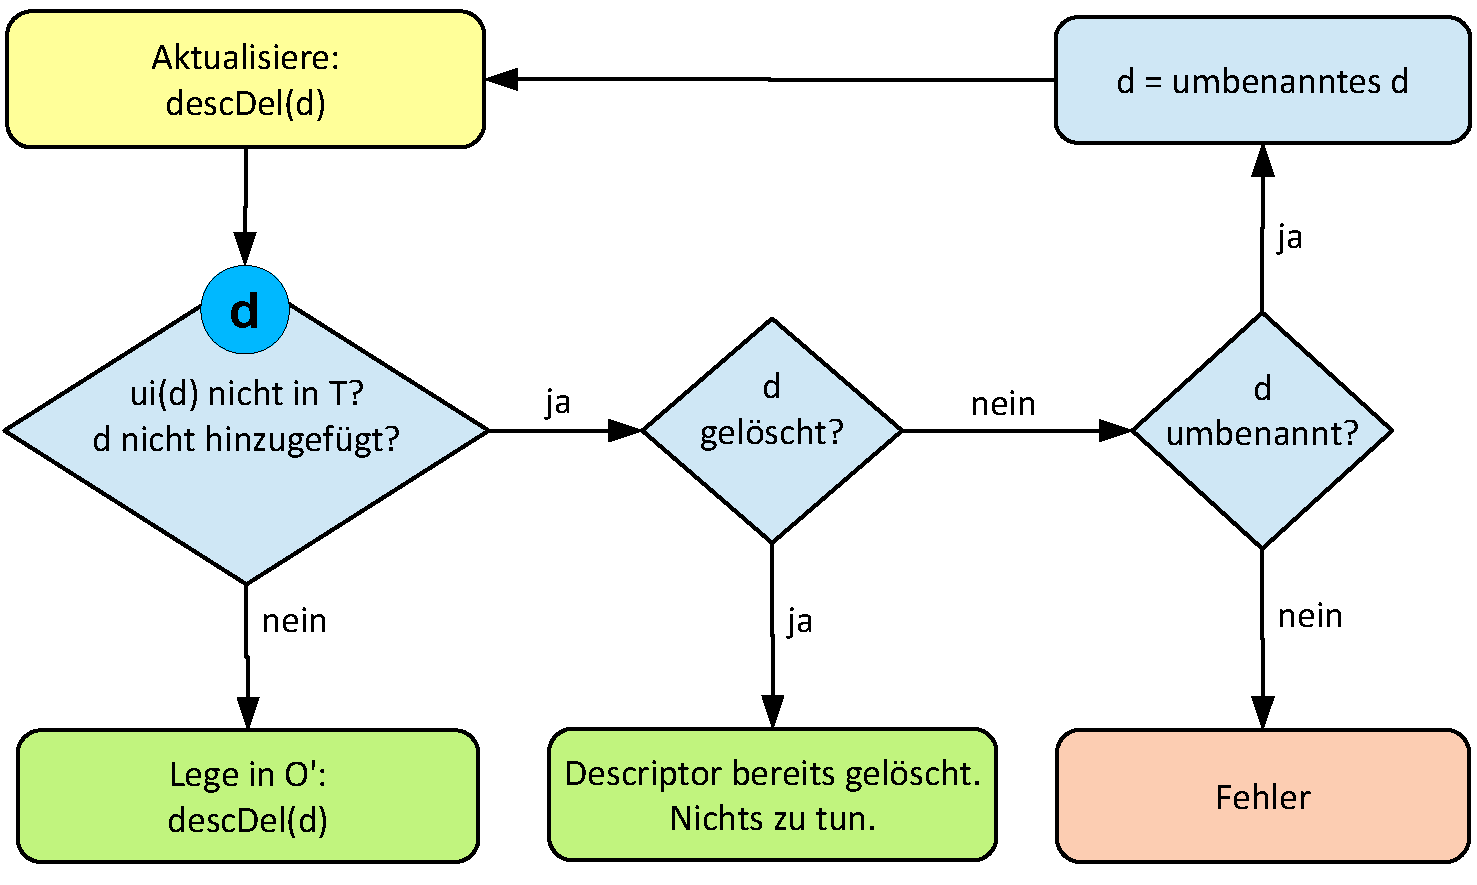
\includegraphics[width=0.8\textwidth]{figs/merge_descDel.pdf}
\end{center}
\caption{Aktualisierung von Descriptor-Löschungen}
\label{figs:merge_descDel}
\end{figure}

\subsubsection{Descriptor-Relabellings und Vertex-Umbenennungen}
Descriptor-Relabellings und Vertex-Umbenennungen treten in diesem Anwendungsfall nicht auf, da keine beim Vergleich des MeSH 2008 und des Semedico-MeSH 2008 bestimmt werden und auch nicht durch das Aktualisieren von Transformationen entstehen können. Daher wurden die beiden Transformationstypen noch nicht umgesetzt.